When developing any hardware architecture, the accompanying software is the key to making
it widely usable without large overheads stemming from custom deployment solutions. Especially
in the \ac{DL} community, there are established tools and workflows that many practitioners
commonly use to develop their neural networks. Therefore, our goal for the software stack
supporting YANA is to provide an end-to-end framework that seamlessly integrates with a wide
range of popular open-source tools for neuromorphic computing.
\begin{figure}[t]
    \centering
    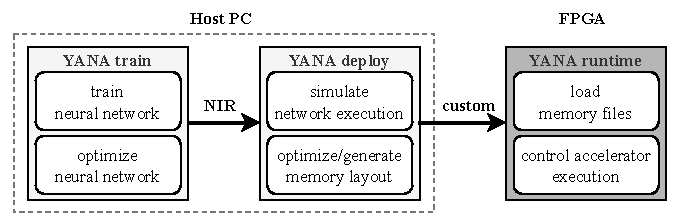
\includegraphics[width=0.9\linewidth]{media/YANA_framework_new.pdf}
    \caption{Overview of the YANA software framework}
    \label{fig:yana-sw-framework}
\end{figure}
Notably, we chose the Neuromorphic Intermediate Representation (NIR) \cite{pedersen_neuromorphic_2024}
as our intermediary format throughout the framework to ensure compatibility with other frameworks for
neuromorphic computing.
The YANA software framework aims
to provide an easy-to-use workflow for hardware-aware training, optimization and deployment \acp{SNN}
targeting our custom neuromorphic accelerator.
It consists of three major modules: YANA train, YANA deploy and YANA runtime, as can be seen in Figure~\ref{fig:yana-sw-framework}. The modules are briefly described as follows:
\\
\textbf{YANA train:}
This module facilitates the training of \acp{SNN} for YANA. Currently, it is based
on the Norse framework~\cite{norse2021}, utilizing additional tools like Tonic~\cite{lenz_gregor_2021_5079802} and
PyTorch Lightning~\cite{Falcon_PyTorch_Lightning_2019}.
Its main addition to Norse is an implementation of YANA's quantized fixed-point \ac{LIF} neuron that includes the \ac{LUT}-based leak calculation.
This allows for hardware-aware training, as the quantization effects and \ac{LUT}-based leak can be directly incorporated into the training process.
Note that the current form of YANA train should be considered
a reference implementation for supporting the \ac{DL} programming model on YANA and can be easily exchanged for any other training framework that supports exporting to NIR.
\\
\textbf{YANA deploy:}
This module handles the translation of trained SNN models into hardware-deployable configurations through several key steps. First, it parses the NIR graph representation and simulates it using the accelerator's fixed-point arithmetic to ensure numeric accuracy. The logical network structure is then transformed into an optimized memory layout that maps individual neurons and weights onto the physical hardware resources.
The module outputs memory configuration files for synapse and routing tables in a custom human-readable format that can be directly loaded onto the accelerator. While currently focusing on dense layers, YANA's native suport for weight sharing provides the foundation for future support of convolutional operations and other structured connectivity patterns.
\\
\textbf{YANA runtime:}
Unlike the previous modules which run on a host computer, the runtime executes directly on the \ac{SoC} FPGA's \ac{PS}. It leverages the PYNQ library~\cite{advanced_micro_devices_inc_pynq_2024} to interface with AMD AXI IPs implemented in the \ac{PL} fabric. The runtime initializes the accelerator with the memory configuration files created by YANA deploy, loads input spike events, and orchestrates the execution sequence. During inference, it tracks performance metrics like execution latency, timestep count, and memory utilization.
The current implementation supports sample-based dataset processing, where complete input samples are preloaded into the accelerator's buffer and processed in batch mode. Future development will introduce stream processing capabilities to enable integration with (event-based) sensors for deployment in real-world scenarios and low-power applications.
